\section{Analysis tasks}\label{sec:analysis-tasks}

In this section, we study a gamut of fundamental analysis tasks, namely function reconstruction
(\autoref{sec:rmse-optimized}), derivative computation (\autoref{sec:gradient} and
\autoref{sec:laplacian}), histogram computation (\autoref{sec:histogram}), and isocontour extraction
(\autoref{sec:isocontour}). For each task, we define an error metric $e$ that is the basis for
evaluating performance of different streams on the task. We use Algorithm~\ref{alg:greedy} to
compute a stream $s_{opt}$ that is optimized for each task. An $s_{sig}$ stream is computed from the
signature of $s_{opt}$. We compare $s_{lvl}$, $s_{bit}$, $s_{wav}$, $s_{mag}$, $s_{sig}$, and
$s_{opt}$ by plotting the error as a function of the number of packets received. To mimic the
effects of entropy compression commonly used in practice, we remove all packets that contain only
leading zero bits from each stream, before plotting. This comparison is performed on a variety of
data sets, listed in \autoref{tbl:data-sets}. \duong{add the discussion about reconstructing the
whole data at full resolution before performing any analysis task.}

\begin{table*}[t]
  \caption{Data sets used in experiments \duong{Update this table}}
  \centering
  \begin{tabular}{p{0.15\linewidth}p{0.20\linewidth}p{0.15\linewidth}p{0.10\linewidth}p{0.15\linewidth}}
  \hline
  Name & Source & Slice dimension & Type & Citation\\
  \hline
  boiler & combustion simulation& $140\times 148$ & float64 &\\
  euler & fluid simulation& $256\times 1024$ & float64 &\\
  kingsnake & CT scan & $1024\times 795$ & uint8 &\\
  plasma & magnetic reconnection simulation& $512\times 512$ & float32 &\\
  marschner-lobb & analytical function& $256\times 256$ & float64 &\\
  diffusivity & hydrodynamics simulation& $384\times 384$ & float64 &\\
  pressure & hydrodynamics simulation& $384\times 384$ & float64 &\\
  velocityz & hydrodynamics simulation& $384\times 384$ & float64 &\\
  turbulence & fluid dynamics simulation& $256\times 256$ & float32 &\\
  \hline
  \end{tabular}\label{tbl:data-sets}
\end{table*}

\subsection{Function reconstruction}\label{sec:rmse-optimized}

The most fundamental analysis task is that of reconstructing the original function itself. The most
common error metric in this case is the root-mean-square error (RMSE). The plots that compare the
streams are in \autoref{fig:rmse-optimized}. The main trend in all cases, is $s_{opt} > s_{sig} >
s_{wav} > s_{bit} > s_{mag} > s_{lvl}$, where ``$>$'' means producing lower RMSE errors.

$s_{bit}$ performs significantly better than $s_{lvl}$, which can be attributed partly to our
removal of leading zero packets. This is because, wavelet coefficients on finer-scale subbands are
much smaller in magnitude. They contain the majority of the leading zero bits, whose removal
benefits $s_{bit}$ the most, as it touches fine-resolution bits the most early. $s_{mag}$
underperforms for the same reason that $s_{lvl}$ does, but to a lesser extent, due to it being
adaptive to the data. $s_{wav}$ outperforms both $s_{lvl}$ and $s_{bit}$, because it follows the
optimal (data-independent) bit ordering in $S_{L,B}$ in the $L_2$ norm, which is also the norm that
the RMSE is based on. $s_{opt}$ unsurprisingly outperforms the rest, being the most data-adaptive.
$s_{sig}$ is the second best stream, as it follows the bit ordering of $s_{opt}$ in $S_{L,B}$. In
general, $s_{wav}$ and $s_{sig}$ are close in performance. In some cases (e.g., \emph{plasma} and
\emph{diffusivity}), the $s_{sig}$ stream is able to adapt more to the data, thus outperforming
$s_{wav}$ by a larger margin.

\begin{figure}[h]
  \centering
	\subcaptionbox{\emph{boiler}}{ {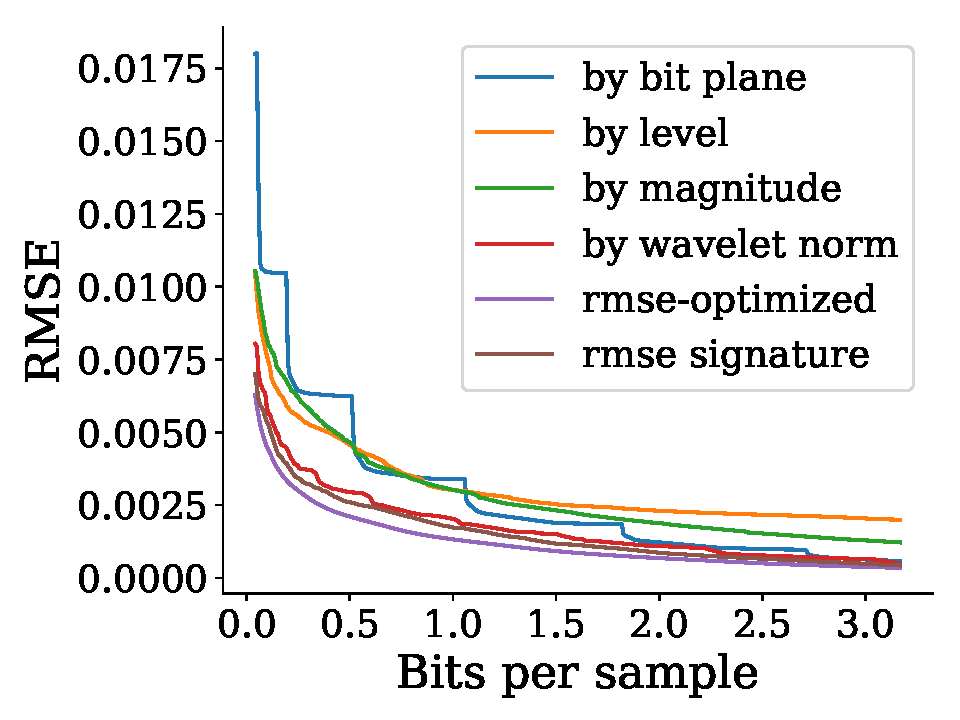
\includegraphics[width=0.48\linewidth]{rmse/rmse-optimized-boiler}}}
		\subcaptionbox{\emph{diffusivity}}{
		{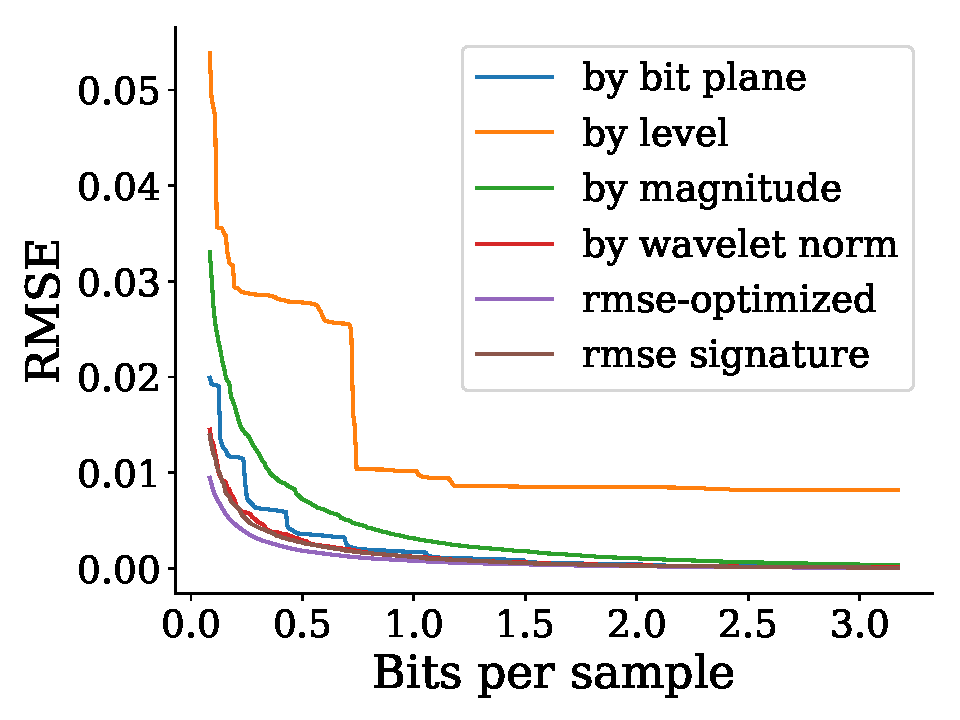
\includegraphics[width=0.48\linewidth]{rmse/rmse-optimized-diffusivity}}}
		\subcaptionbox{\emph{plasma}}{ {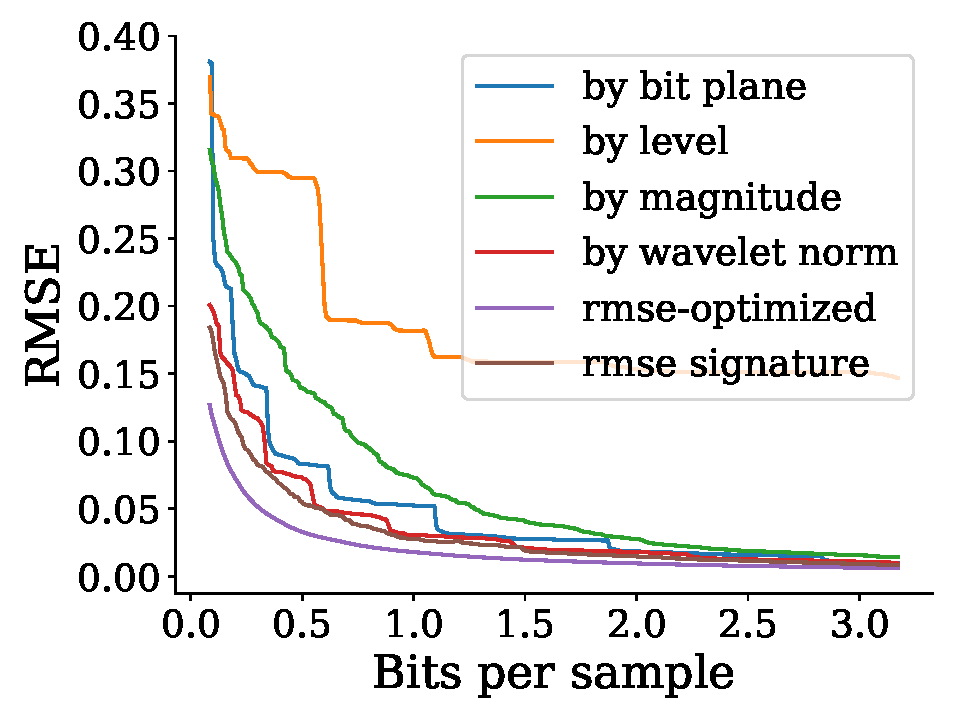
\includegraphics[width=0.48\linewidth]{rmse/rmse-optimized-plasma}}}
		\subcaptionbox{\emph{turbulence}}{
		{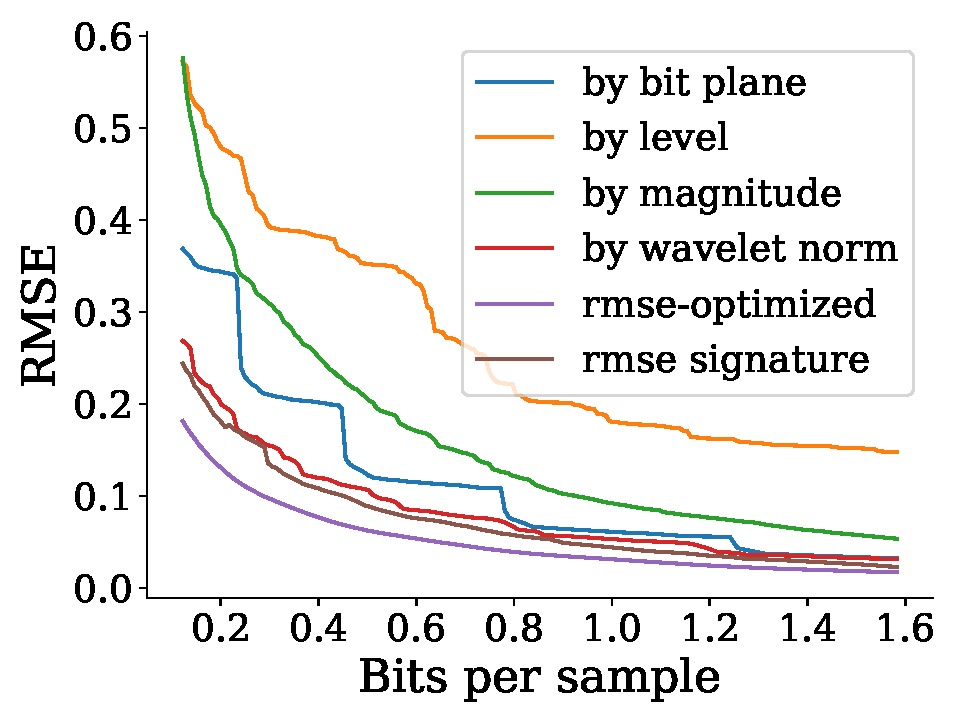
\includegraphics[width=0.48\linewidth]{rmse/rmse-optimized-turbulence}}}
		\caption{Root-mean-square error of reconstructed functions for different streams and data sets.
		Lower is better. The streams are truncated to highlight the differences, without omitting
		important information. Leading zero packets are not used for plotting. In all cases, the
		ordering of performance, from best to worst, is $s_{opt} > s_{sig} > s_{wav} > s_{bit} > s_{mag}
		> s_{lvl}$.}\label{fig:rmse-optimized}
\end{figure}

In \autoref{fig:rmse-rendering} we volume render the \emph{plasma} data set at 0.1 bits per sample,
for all streams. Bits per sample (bps) are calculated by dividing the total size of received packets
(in bits) by the total number of samples. Although $s_{lvl}$ has the precision to obtain an accurate
background, it lacks resolution to resolve the fine details. $s_{bit}$, instead, lacks the precision
to reconstruct the (mostly smooth) background, but has enough resolution to capture the fine details
well. $s_{wav}$ balances both precision and resolution, producing a more accurate picture as a
whole. In this case, the $s_sig$ stream manages to produce the most accurate rendering. In general,
$s_{sig}$ benefits more from ``anisotropic'' data, such as \emph{plasma}, where most features lie on
a thin ``surface''. For such data, wavelet coefficients along one dimension are often larger in
magnitude compared to those along other dimensions, which $s_{opt}$, and hence $s_{sig}$, can take
advantage of, but not $s_{wav}$.

\begin{figure}[h]
	\centering
	\subcaptionbox{\emph{by level} ($s_{lvl}$)}{
	{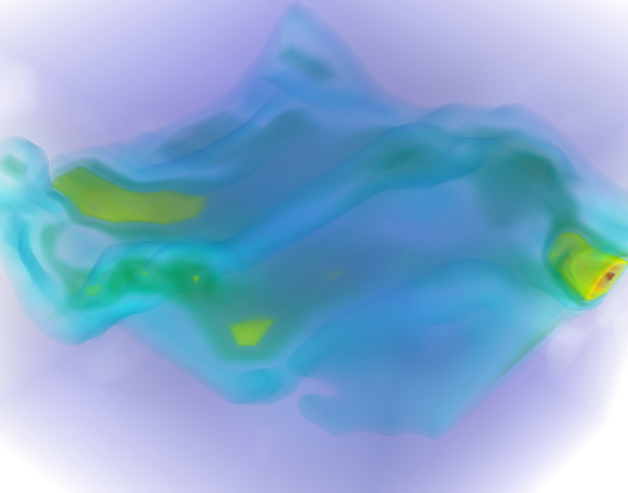
\includegraphics[width=0.31\linewidth]{rmse/rmse-plasma-level}}} \subcaptionbox{\emph{by bit
	plane ($s_{bit}$)}}{ {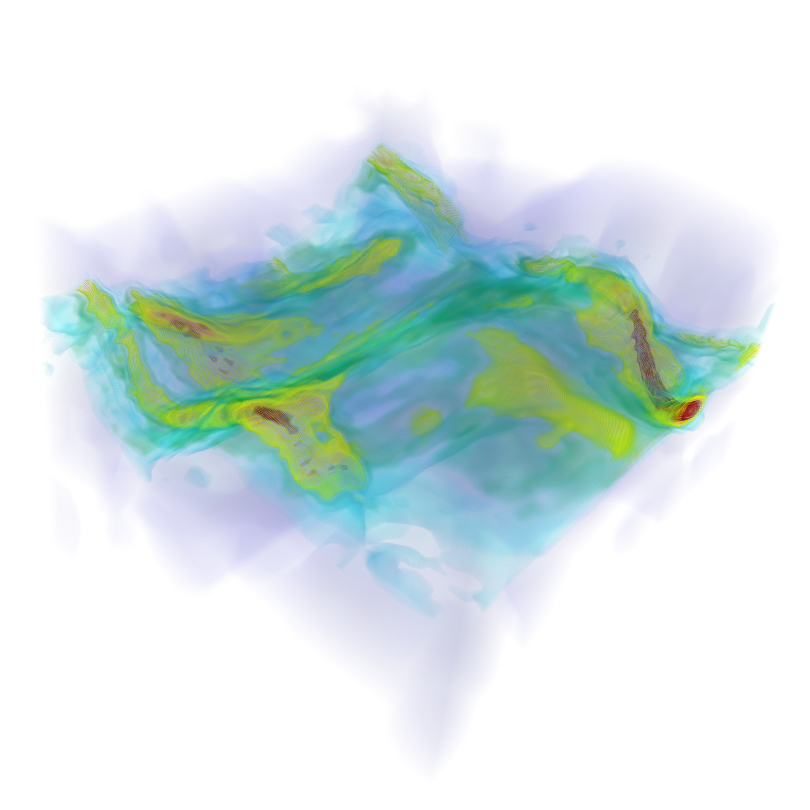
\includegraphics[width=0.31\linewidth]{rmse/rmse-plasma-bit-plane}}}
	\subcaptionbox{\emph{by magnitude ($s_{mag}$)}}{
	{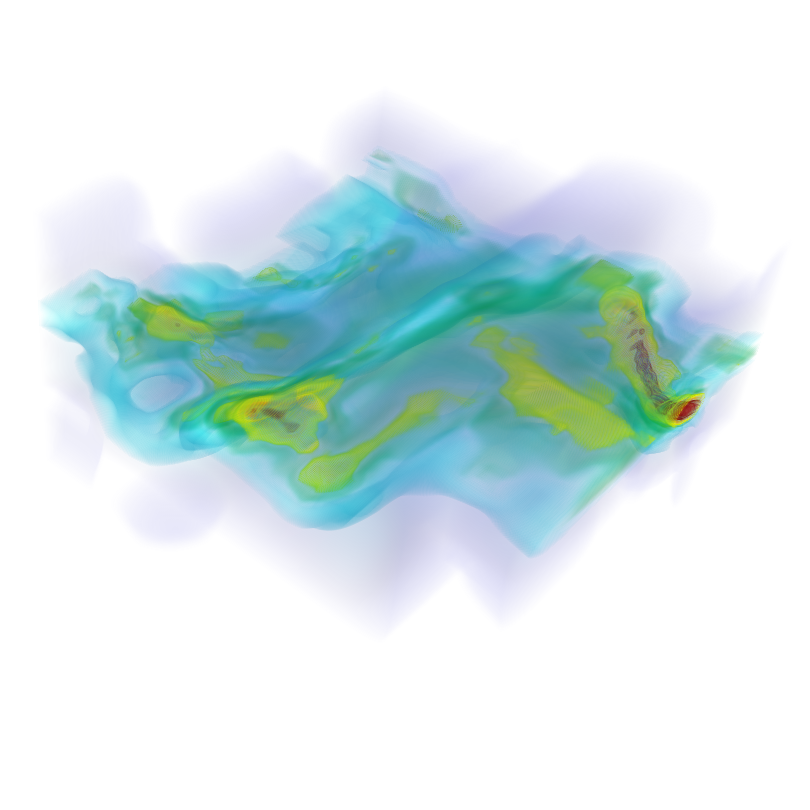
\includegraphics[width=0.31\linewidth]{rmse/rmse-plasma-magnitude}}} \subcaptionbox{\emph{by
	wavelet norm ($s_{wav}$)}}{
	{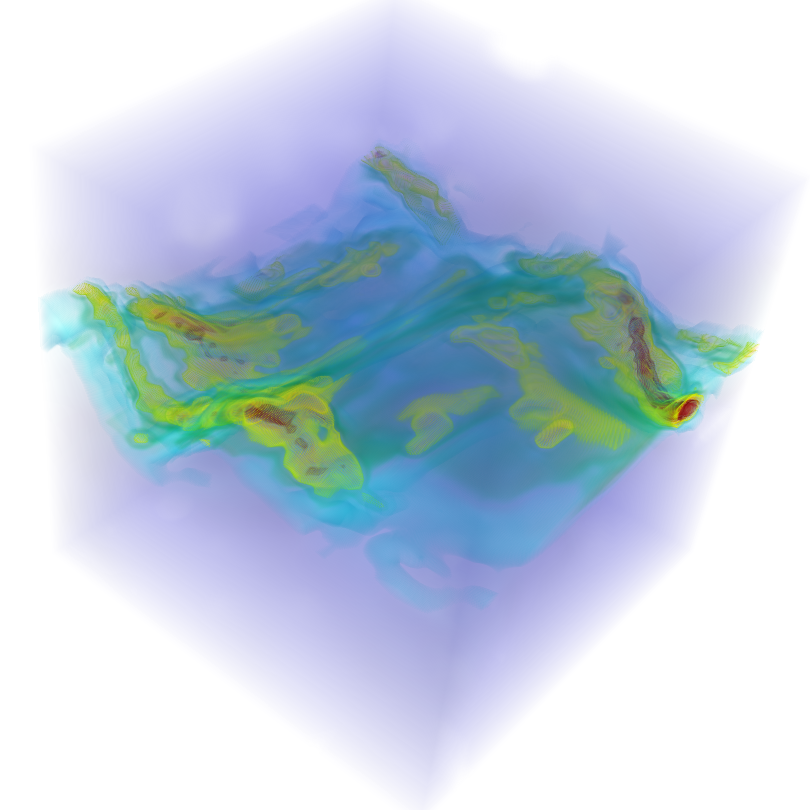
\includegraphics[width=0.31\linewidth]{rmse/rmse-plasma-wavelet-norm}}} \subcaptionbox{\emph{by
	signature ($s_{sig}$)}}{ {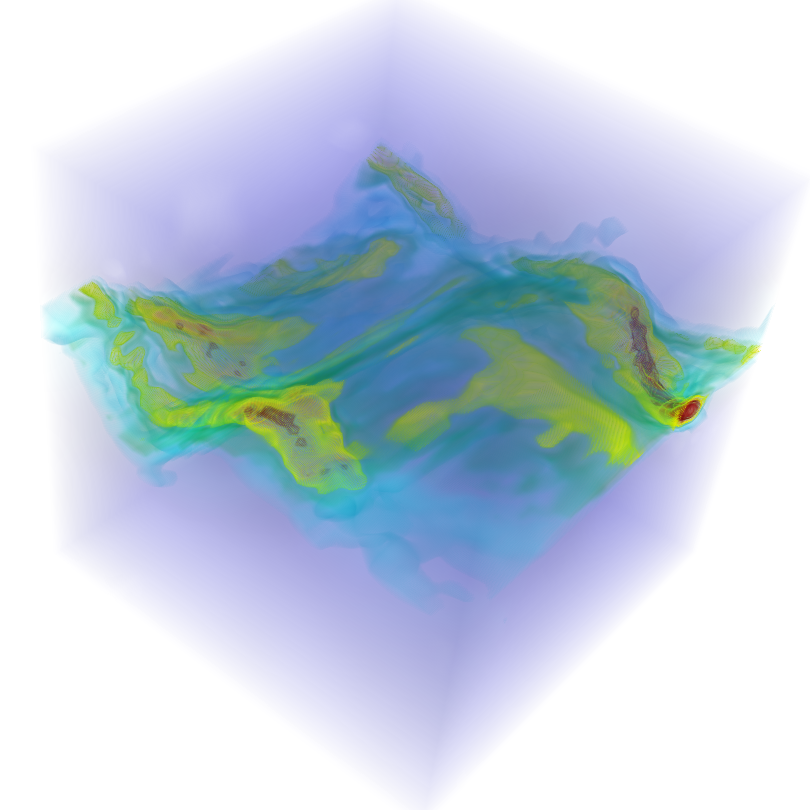
\includegraphics[width=0.31\linewidth]{rmse/rmse-plasma-signature}}}
	\subcaptionbox{\emph{reference}}{
	{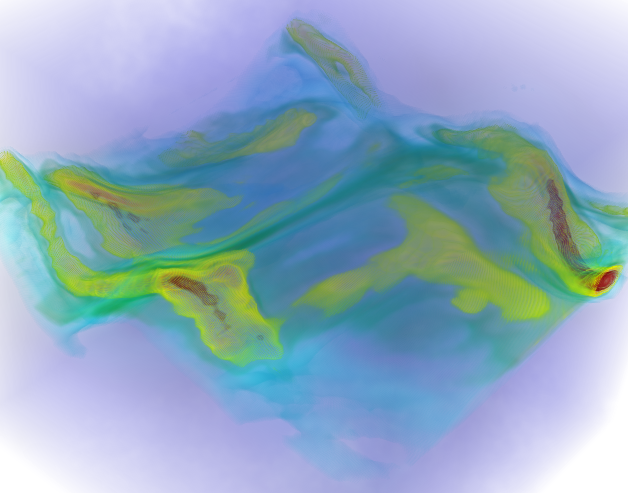
\includegraphics[width=0.31\linewidth]{rmse/rmse-plasma-groundtruth}}} \caption{Volume renderings
	of a $64^3$ region of \emph{plasma} at 0.1 bps. $s_{lvl}$ captures the background (purple-blue)
	well, while $s_{bit}$ captures the fine details better. $s_{wav}$ combines the strength of both.
	$s_{sig}$, however, produces the most accurate rendering (compare, e.g., yellow
	features).}\label{fig:rmse-rendering}
\end{figure}
